% SPDX-FileCopyrightText: 2026 Onur Tuncer and Stereon contributors
% SPDX-License-Identifier: MPL-2.0
%
% This Source Code Form is subject to the terms of the Mozilla Public
% License, v. 2.0. If a copy of the MPL was not distributed with this
% file, You can obtain one at https://mozilla.org/MPL/2.0/.
%
% Coaxial surfaces of revolution (docs/intersection.rst, Elementary
% surfaces). In the meridian half-plane (rho, z) a torus is a circle about
% (R, z_c), a cylinder the line rho = r, a plane across the axis the line
% z = h, a cone two lines through its apex. Each point where two profiles
% meet turns about the axis into a circle of the intersection: crossings
% (filled) into transverse circles, the touch of the cylinder's line with
% the torus's circle (open) into a circle of tangency, the fillet's case.
\documentclass[tikz,border=6pt]{standalone}
\usetikzlibrary{arrows.meta}
\definecolor{torus}{RGB}{31,119,180}
\definecolor{cyl}{RGB}{255,127,14}
\definecolor{flat}{RGB}{44,160,44}
\definecolor{cone}{RGB}{148,103,189}
\begin{document}
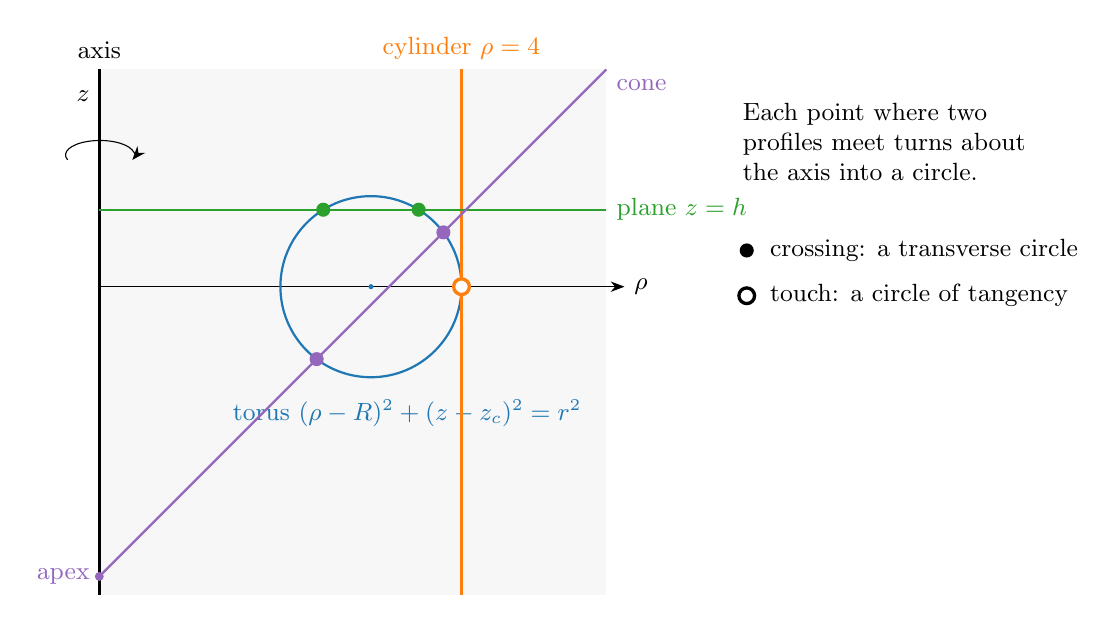
\begin{tikzpicture}[scale=1.15,lbl/.style={font=\small},
    cross/.style={circle,fill,inner sep=1.8pt},
    touch/.style={circle,draw,very thick,fill=white,inner sep=2pt}]
  % The half-plane and the axis
  \fill[black!3] (0,-3.4) rectangle (5.6,2.4);
  \draw[very thick] (0,-3.4) -- (0,2.4) node[lbl,above] {axis};
  \draw[-{Stealth[length=5pt]}] (0,0) -- (5.8,0) node[lbl,right] {$\rho$};
  \node[lbl,left] at (0,2.1) {$z$};
  % Torus: circle about (3, 0), radius 1
  \draw[torus,thick] (3,0) circle (1);
  \fill[torus] (3,0) circle (0.8pt);
  \node[lbl,torus] at (3.4,-1.4) {torus $(\rho - R)^2 + (z - z_c)^2 = r^2$};
  % Cylinder: rho = 4, tangent to the torus at (4, 0)
  \draw[cyl,thick] (4,-3.4) -- (4,2.4) node[lbl,above] {cylinder $\rho = 4$};
  \node[touch,draw=cyl] at (4,0) {};
  % Plane across the axis: z = 0.85, crossing the torus twice
  \draw[draw=flat,thick] (0,0.85) -- (5.6,0.85) node[lbl,right,flat] {plane $z = h$};
  \node[cross,flat] at ({3-sqrt(1-0.85^2)},0.85) {};
  \node[cross,flat] at ({3+sqrt(1-0.85^2)},0.85) {};
  % Cone: apex on the axis at z = -3.2, half-angle 45 degrees
  \pgfmathsetmacro{\k}{tan(45)}
  \draw[cone,thick] (0,-3.2) -- (5.6,{5.6/\k-3.2}) node[lbl,below right] {cone};
  \fill[cone] (0,-3.2) circle (1.4pt) node[lbl,left] {apex};
  % Its crossings with the torus's circle
  \foreach \s in {-1,1} {
    % Points on rho = k (z + 3.2) at distance 1 from (3, 0).
    \pgfmathsetmacro{\a}{1+\k*\k}
    \pgfmathsetmacro{\b}{2*(\k*\k*3.2-3*\k)}
    \pgfmathsetmacro{\c}{(\k*3.2-3)^2-1}
    \pgfmathsetmacro{\z}{(-\b+\s*sqrt(\b*\b-4*\a*\c))/(2*\a)}
    \node[cross,cone] at ({\k*(\z+3.2)},\z) {};
  }
  % The turn
  \draw[-{Stealth[length=5pt]},thin] (-0.35,1.4) arc[start angle=200,end angle=-20,x radius=0.38,y radius=0.16];
  \node[lbl,align=left,anchor=west] at (7.0,1.6) {Each point where two\\profiles meet turns about\\the axis into a circle.};
  \node[cross] at (7.15,0.4) {};
  \node[lbl,anchor=west] at (7.3,0.4) {crossing: a transverse circle};
  \node[touch] at (7.15,-0.1) {};
  \node[lbl,anchor=west] at (7.3,-0.1) {touch: a circle of tangency};
\end{tikzpicture}
\end{document}
